%%%%%%%%%%%%%%%%%%%%%%%%%%%%%%%%%%%%%%%%%%%%%%%%%%%%
% LECTURE 24: THERMAL RADIATION (CONTINUED)
%%%%%%%%%%%%%%%%%%%%%%%%%%%%%%%%%%%%%%%%%%%%%%%%%%%%
\section*{Wave vs. Particle Nature of Light}
\addcontentsline{toc}{section}{Wave vs. Particle Nature of Light}

Historically, there has been debate about the nature of light:
\begin{itemize}
    \item Newton favored the particle theory
    \item Maxwell's equations supported the wave theory
    \item Einstein later proposed the wave-particle duality concept
    \item Modern physics has developed a more comprehensive understanding beyond simple duality
\end{itemize}

For thermal radiation analysis, we need to switch between wave and particle descriptions depending on the phenomenon being explained. This helps us better understand the various terminologies and processes involved in radiation heat transfer.

%%%%%%%%%%%%%%%%%%%%%%%%%%%%%%%%%%%%%%%%%%%%%%%%%%%%
\subsection*{Radiation Heat Fluxes}
\addcontentsline{toc}{subsection}{Radiation Heat Fluxes}
%%%%%%%%%%%%%%%%%%%%%%%%%%%%%%%%%%%%%%%%%%%%%%%%%%%%

\subsubsection*{Direction-Based Terminology}
\addcontentsline{toc}{subsubsection}{Direction-Based Terminology}

Similar to conduction heat transfer where we track heat from generation to dissipation, radiation heat transfer requires us to track the path of energy. We define key terms based on directional behavior:
%
\begin{figure}[H]
    \centering
    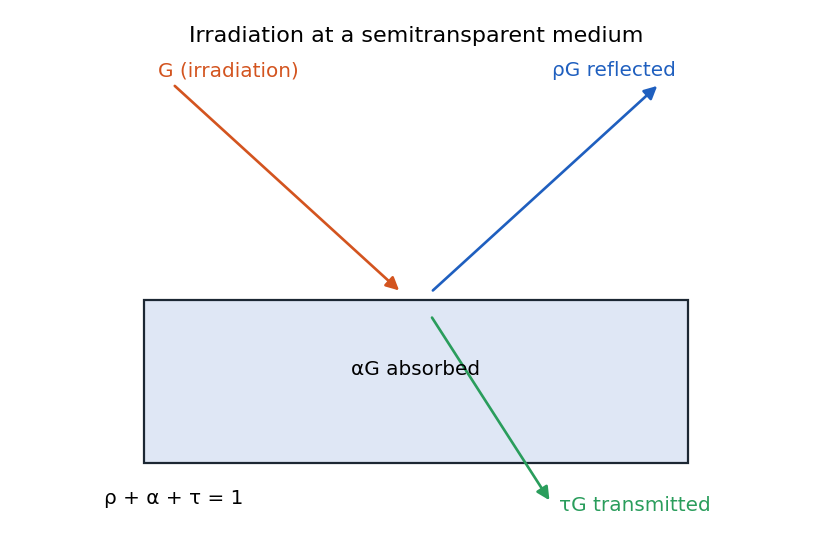
\includegraphics[width=0.8\linewidth]{pics/irradiation.png}
    \caption{Radiation at a surface. (a) Reflection, absorption, and transmission of irradiation for a
semitransparent medium. (b) The radiosity for an opaque medium.}
\end{figure}
%
\begin{itemize}
    \item \textbf{Irradiation ($G$)}: Rate of incident radiation per unit area. Incoming radiation from external sources that lands on a surface (W/m$^2$).
    \item \textbf{Reflection ($G_{ref}$)}: Portion of irradiation that bounces back from the surface (W/m$^2$).
    \item \textbf{Absorption ($G_{abs}$)}: Portion of irradiation that is captured by the material near the surface (W/m$^2$).
    \item \textbf{Transmission ($G_{tr}$)}: Portion of irradiation that passes through the material (for semi-transparent media) (W/m$^2$)

    For energy conservation in semi-transparent media:
        \[
        G = G_{ref} + G_{abs} + G_{tr}
        \]

    For opaque materials (no transmission):
        \[
        G = G_{ref} + G_{abs}
        \]
    \item \textbf{Emission ($E$)}: Rate of energy emission per unit area. It is separate from irradiation processes, as it represents energy originating from within the material itself due to its temperature. It has no direct relationship with the incoming irradiation (W/m$^2$).
    \[  
                E = \varepsilon \sigma T^4_s        
    \]
    \item \textbf{Radiosity ($J$)}: Rate of incident radiation per unit area . It represents the total radiation leaving a surface, combining both reflection and emission (W/m$^2$):
    \[
        J = G_{ref} + E
    \]
    \item \textbf{Net Radiation Heat Flux ($q''_{\text{rad}}$}): is a scalar quantity representing the rate of energy transfer per unit area leaving the surface:
        \[
                q''_{\text{rad}} = J - G
        \]
\end{itemize}

Note that "emissive power" is somewhat of a misnomer, as it's actually power per unit area (power density), not merely power.

%%%%%%%%%%%%%%%%%%%%%%%%%%%%%%%%%%%%%%%%%%%%%%%%%%%%
\subsection*{Radiative Properties}
\addcontentsline{toc}{subsection}{ Radiative Properties}
%%%%%%%%%%%%%%%%%%%%%%%%%%%%%%%%%%%%%%%%%%%%%%%%%%%%

From a quantum/particle perspective, radiative properties like reflectivity, absorptivity, and transmissivity can be understood as probabilities:
%
\[
    \begin{aligned}
     G &=G_{\text {ref }}+G_{\text {abs }}+G_{\text {tr }} 
    \\[0.5em]
    1 &=\frac{G_{\text {ref }}}{G}+\frac{G_{\text {abs }}}{G}+\frac{G_{\text {tr }}}{G} 
    \\[0.5em]
    \quad 1 &=\rho+\alpha+\tau
    \end{aligned}
\]
where,
\begin{itemize}
    \item \textbf{Reflectivity ($\rho$)}: Probability that a photon will be reflected at the surface
    \item \textbf{Absorptivity ($\alpha$)}: Probability that a photon will be absorbed by the material
    \item \textbf{Transmissivity ($\tau$)}: Probability that a photon will pass through the material
\end{itemize}
%
This probabilistic interpretation helps explain why these properties can depend on:
\begin{itemize}
    \item Direction of incoming photon
    \item Wavelength (color) of the photon
    \item Material properties
\end{itemize}
%
For obaque material ($\tau =0$) which means $\rho = 1- \alpha$:
\[
    \begin{aligned}
        q_{\text {rad }}^{\prime \prime} & = J - G
        \\[0.5em]
        q_{\text {rad }}^{\prime \prime} & = E + G_{ref} - G
        \\[0.5em]
        q_{\text {rad }}^{\prime \prime} & = E + \rho G - G
        \\[0.5em]
        q_{\text {rad }}^{\prime \prime} & = \underbrace{\varepsilon \sigma T_s^4}_{\textit{outbound}}- \underbrace{\alpha G}_{\textit{inbound}}
    \end{aligned}
\]
%
\begin{table}[ht]
  \centering
  \caption{Radiative Flux Quantities}
  \label{tab:radiative_flux}
  % tweak row spacing
  \renewcommand{\arraystretch}{1.2}
  \begin{tabular}{@{}
      >{\raggedright\arraybackslash}p{3cm}  % Flux
      >{\raggedright\arraybackslash}p{7cm}  % Description
      >{\raggedright\arraybackslash}p{4cm}  % Comment
    @{}}
    \toprule
    \textbf{Flux (W/m$^2$)} 
      & \textbf{Description} 
      & \textbf{Comment} \\
    \midrule
    Emissive power, $E$
      & Rate at which radiation is emitted from a surface per unit area
      & $E = \varepsilon\,\sigma\,T_s^{4}$ \\[1ex]

    Irradiation, $G$
      & Rate at which radiation is incident upon a surface per unit area
      & Irradiation can be reflected, absorbed, or transmitted \\[1ex]

    Radiosity, $J$
      & Rate at which radiation leaves a surface per unit area
      & For an opaque surface: $J = E + \rho\,G$ \\[1ex]

    Net radiative flux, $q''_{\mathrm{rad}} = J - G$
      & Net rate of radiation leaving a surface per unit area
      & For an opaque surface: $q''_{\mathrm{rad}} = \varepsilon\,\sigma\,T_s^{4} - \alpha\,G$ \\
    \bottomrule
  \end{tabular}
\end{table}
%%%%%%%%%%%%%%%%%%%%%%%%%%%%%%%%%%%%%%%%%%%%%%%%%%%%
\subsection*{Radiation and Irradiation density}
\addcontentsline{toc}{subsection}{Radiation and Irradiation density}
%%%%%%%%%%%%%%%%%%%%%%%%%%%%%%%%%%%%%%%%%%%%%%%%%%%%

Temperature alone is insufficient to characterize radiation, as the distribution across wavelengths and directions is crucial. This leads to the concept of intensity.

\paragraph{Radiation Intensity} is defined as heat flux per unit solid angle per unit wavelength:
\[
I_{\lambda,e}(\lambda,\theta,\phi) = \frac{dq}{dA_1 \cdot \cos\theta \cdot d\omega \cdot d\lambda} \left[\frac{\text{W}}{\text{m}^2 \cdot \text{sr} \cdot \mu\text{m}}\right]
\]
%
\begin{figure}[H]
    \centering
    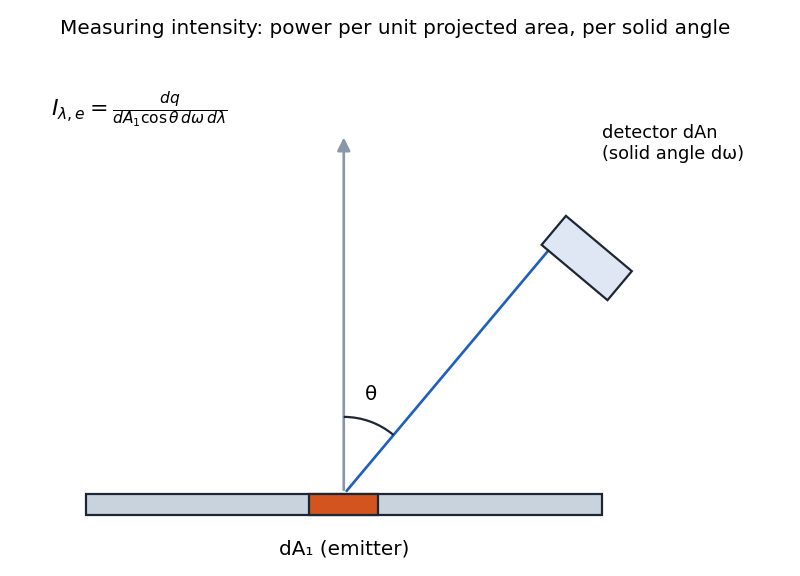
\includegraphics[width=0.4\linewidth]{pics/measure_Intensity.png}
\end{figure}
%

Where:
\begin{itemize}
    \item $dq$ is the energy rate
    \item $dA_1$ is the surface area element
    \item $\cos\theta$ accounts for the projected area
    \item $d\omega$ is the solid angle element
    \item $d\lambda$ is the wavelength interval
\end{itemize}

This definition includes:
\begin{itemize}
    \item $\cos\theta$ factor to account for projected area
    \item Solid angle to measure the angular spread
    \item Wavelength interval for spectral distribution
\end{itemize}

The units of intensity are W/(m$^2$·sr·$\mu$m), where "sr" represents steradian (solid angle unit) and "$\mu$m" represents the wavelength unit.
%
\[
        I_{\lambda ,e}(\lambda, \theta, \phi) \rightarrow
        \left\{
            \begin{array}{l}
                \text{spectral} \propto (\lambda) 
                \\
                 \text{directional} \propto (\theta, \phi)
            \end{array}
        \right.
\]
%
\paragraph{Irradiation Intensity} is defined similarly for incoming radiation:

\[
I_{\lambda,i}(\lambda,\theta,\phi) = \frac{dq_{\text{incident}}}{dA_1 \cos\theta \cdot d\omega\cdot d\lambda} \left[\frac{\text{W}}{\text{m}^2 \cdot \text{sr} \cdot \mu\text{m}}\right]
\]

Note: Intensity should not be confused with brightness, which is a different concept related to perception.

%%%%%%%%%%%%%%%%%%%%%%%%%%%%%%%%%%%%%%%%%%%%%%%%%%%%
\subsection*{Qualifiers on Surface Properties}
\addcontentsline{toc}{subsection}{Qualifiers on Surface Properties}
%%%%%%%%%%%%%%%%%%%%%%%%%%%%%%%%%%%%%%%%%%%%%%%%%%%%

Surface properties such as emissivity ($\varepsilon$), absorptivity ($\alpha$), reflectivity ($\rho$), and transmissivity ($\tau$) can depend on:

\begin{itemize}
    \item Wavelength ($\lambda$)
    \item Direction, defined by angles $\theta$ and $\phi$
\end{itemize}

To describe this dependence, we use specific qualifiers:

\begin{itemize}
    \item \textbf{Spectral}: Indicates dependence on wavelength $\lambda$
    \item \textbf{Total}: Indicates integration over all wavelengths
    \item \textbf{Directional}: Indicates dependence on direction ($\theta$, $\phi$)
    \item \textbf{Hemispherical}: Indicates integration over all directions
\end{itemize}

\noindent
Here are some examples:

\begin{itemize}
    \item \textbf{Hemispherical total emissivity:} $\bar{\varepsilon}$ \\
    (Independent of both wavelength and direction)

    \item \textbf{Hemispherical spectral emissivity:} $\varepsilon_\lambda$ \\
    (Depends on $\lambda$, integrated over all angles)

    \item \textbf{Directional spectral absorptivity:} $\alpha_{\lambda, \theta, \phi}$ \\
    (Depends on both $\lambda$ and direction)
\end{itemize}



%%%%%%%%%%%%%%%%%%%%%%%%%%%%%%%%%%%%%%%%%%%%%%%%%%%%
\subsection*{Integrated Radiative Quantities}
\addcontentsline{toc}{subsection}{Integrated Radiative Quantities}
%%%%%%%%%%%%%%%%%%%%%%%%%%%%%%%%%%%%%%%%%%%%%%%%%%%%

For engineering calculations, intensity is often integrated over direction and/or wavelength to obtain simpler quantities.

\paragraph{Spectral Hemispherical Flux} is the intensity integrated over all directions in the hemisphere:
\[
    \begin{array}{ll}
        \text{emission} &  E_{\lambda}(\lambda) =  q''_{\lambda}(\lambda)= \int_0^{2\pi} \int_0^{\pi/2} I_{\lambda,e}(\lambda,\theta,\phi) \sin\theta \cos\theta \, d\theta \, d\phi \left[\frac{\text{W}}{\text{m}^2 \cdot \mu\text{m}}\right]
        \\[1.5em]
        \text{irradiation} & G_{\lambda}(\lambda) = \int_0^{2\pi} \int_0^{\pi/2} I_{\lambda,i}(\lambda,\theta,\phi) \sin\theta \cos\theta \, d\theta \, d\phi \left[\frac{\text{W}}{\text{m}^2 \cdot \mu\text{m}}\right]
    \end{array}
\]

\paragraph{Total Heat Flux} is the spectral quantity integrated over all wavelengths:
\[
    \begin{array}{ll}
        \text{emission} &  E = q'' = \int_0^{\infty} E_{\lambda}(\lambda) \, d\lambda \left[\frac{\text{W}}{\text{m}^2}\right]
        \\[1.5em]
        \text{irradiation} & G = \int_0^{\infty} G_{\lambda}(\lambda) \, d\lambda \left[\frac{\text{W}}{\text{m}^2}\right]
    \end{array}
\]


%%%%%%%%%%%%%%%%%%%%%%%%%%%%%%%%%%%%%%%%%%%%%%%%%%%%
\subsection*{Diffuse Surfaces and Radiation}
\addcontentsline{toc}{subsection}{Diffuse Surfaces and Radiation}
%%%%%%%%%%%%%%%%%%%%%%%%%%%%%%%%%%%%%%%%%%%%%%%%%%%%

A surface is called \textbf{diffuse} if its radiation intensity is uniform in all directions:
%
For diffuse emission:
\[
    I_{\lambda,e}(\lambda,\theta,\phi) = I_{\lambda,e}(\lambda) \quad \text{(independent of $\theta$ and $\phi$)}
\]
%
For diffuse irradiation:
\[
    I_{\lambda,i}(\lambda,\theta,\phi) = I_{\lambda,i}(\lambda) \quad \text{(independent of $\theta$ and $\phi$)}
\]
%
Therefore,
%
\[
    \begin{array}{ll}
        \text{emission} &  E_{\lambda}(\lambda) =  q''_{\lambda}(\lambda)= \textcolor{red}{I_{\lambda,e}(\lambda)} \int_0^{2\pi} \int_0^{\pi/2} \sin\theta \cos\theta \, d\theta \, d\phi  
        \\[1.5em]
        &  E_{\lambda}(\lambda) = I_{\lambda,e} \pi \ \left[\frac{\text{W}}{\text{m}^2 \cdot \mu\text{m}}\right]
        \\[1.5em]
        \text{irradiation} & G_{\lambda}(\lambda) = \textcolor{red}{I_{\lambda,i}(\lambda)}\int_0^{2\pi} \int_0^{\pi/2}  \sin\theta \cos\theta \, d\theta \, d\phi
        \\[1.5em]
        & G_{\lambda}(\lambda) = I_{\lambda,i}\pi \ \left[\frac{\text{W}}{\text{m}^2 \cdot \mu\text{m}}\right]
    \end{array}
\]
%
When a problem is described as "diffuse," it typically means both the surface emission and irradiation are assumed to be diffuse.
%%%%%%%%%%%%%%%%%%%%%%%%%%%%%%%%%%%%%%%%%%%%%%%%%%%%%%
\subsubsection*{Relationship Between Intensity and Flux for Diffuse Radiation}
\addcontentsline{toc}{subsubsection}{Relationship Between Intensity and Flux for Diffuse Radiation}
%%%%%%%%%%%%%%%%%%%%%%%%%%%%%%%%%%%%%%%%%%%%%%%%%%%%%%
For diffuse surfaces, the integration simplifies:

\begin{definition}  
\[
    \begin{aligned}
        E &= \int_0^{\infty} E_{\lambda} \, d\lambda 
           = \int_0^{\infty} I_{\lambda,e}(\lambda) \underbrace{\left(\int_0^{2\pi} \int_0^{\pi/2}  \sin\theta \cos\theta \, d\theta \, d\phi \right) }_{\pi}\, d\lambda  
           = \int_0^{\infty} I_{\lambda,e}\,\pi \, d\lambda
        \\[1em]
        E &= \pi I_e \ \left[\frac{\text{W}}{\text{m}^2}\right]
    \end{aligned}
\]
%
Similarly:
\[
G = \pi I_i \ \left[\frac{\text{W}}{\text{m}^2}\right]
\]

Also for total radiosity ($J$):
\[
    J = E + \rho G = \pi I_e + \pi \;\overbrace{\rho I_i}^{I_r} = \pi (I_e + I_r) = \pi I_{e+r}
\]
\end{definition}
%%%%%%%%%%%%%%%%%%%%%%%%%%%%%%%%%%%%%%%%%%%%%%%%%%%%
\subsubsection*{Special Notes}
\addcontentsline{toc}{subsubsection}{Special Notes}
%%%%%%%%%%%%%%%%%%%%%%%%%%%%%%%%%%%%%%%%%%%%%%%%%%%%

\begin{itemize}
  \item Intensities are defined based on \emph{normal area} 
    (i.e., include a $1/\cos\theta$ term in the definitions).
  \item Fluxes are defined based on \emph{actual surface area} 
    (i.e., include a $\cos\theta$ term in integrations).
  \item In this class, we usually assume:
    \begin{enumerate}[label=\roman*)]
      \item diffuse emission,
      \item diffuse reflection, and
      \item diffuse irradiation, with or without spectral distributions.
    \end{enumerate}
\end{itemize}



% %%%%%%%%%%%%%%%%%%%%%%%%%%%%%%%%%%%%%%%%%%%%%%%%%%%%
% \subsection*{Radiative Properties}
% \addcontentsline{toc}{subsection}{Radiative Properties}
% %%%%%%%%%%%%%%%%%%%%%%%%%%%%%%%%%%%%%%%%%%%%%%%%%%%%

% \subsubsection*{Absorptivity}
% \addcontentsline{toc}{subsubsection}{Absorptivity}

% Absorptivity represents the fraction of incident radiation that is absorbed by a surface:

% Spectral, directional absorptivity:
% \[
% \alpha_{\lambda,\theta}(\lambda,\theta,\phi) = \frac{I_{\lambda,i,abs}(\lambda,\theta,\phi)}{I_{\lambda,i}(\lambda,\theta,\phi)}
% \]

% Spectral, hemispherical absorptivity:
% \[
% \alpha_{\lambda} = \frac{G_{\lambda,abs}(\lambda)}{G_{\lambda}(\lambda)}
% \]

% Total, hemispherical absorptivity:
% \[
% \alpha = \frac{G_{abs}}{G}
% \]

% Important note: Absorptivity is determined by both the surface properties and the incident radiation characteristics.

% \subsubsection*{Reflectivity}
% \addcontentsline{toc}{subsubsection}{Reflectivity}

% Reflectivity represents the fraction of incident radiation that is reflected by a surface:

% Spectral, directional reflectivity:
% \[
% \rho_{\lambda,\theta}(\lambda,\theta,\phi) = \frac{I_{\lambda,i,ref}(\lambda,\theta,\phi)}{I_{\lambda,i}(\lambda,\theta,\phi)}
% \]

% Spectral, hemispherical reflectivity:
% \[
% \rho_{\lambda} = \frac{G_{\lambda,ref}(\lambda)}{G_{\lambda}(\lambda)}
% \]

% Total, hemispherical reflectivity:
% \[
% \rho = \frac{G_{ref}}{G}
% \]

% \subsubsection*{Transmissivity}
% \addcontentsline{toc}{subsubsection}{Transmissivity}

% Transmissivity represents the fraction of incident radiation that passes through a material:

% Spectral, directional transmissivity:
% \[
% \tau_{\lambda,\theta}(\lambda,\theta,\phi) = \frac{I_{\lambda,i,tr}(\lambda,\theta,\phi)}{I_{\lambda,i}(\lambda,\theta,\phi)}
% \]

% Spectral, hemispherical transmissivity:
% \[
% \tau_{\lambda} = \frac{G_{\lambda,tr}(\lambda)}{G_{\lambda}(\lambda)}
% \]

% Total, hemispherical transmissivity:
% \[
% \tau = \frac{G_{tr}}{G}
% \]

% \subsubsection*{Conservation Relationships}
% \addcontentsline{toc}{subsubsection}{Conservation Relationships}

% For semi-transparent media:
% \[
% \rho_{\lambda} + \alpha_{\lambda} + \tau_{\lambda} = 1 \quad \text{(spectral)}
% \]
% \[
% \rho + \alpha + \tau = 1 \quad \text{(total)}
% \]

% For opaque media:
% \[
% \rho_{\lambda} + \alpha_{\lambda} = 1 \quad \text{(spectral)}
% \]
% \[
% \rho + \alpha = 1 \quad \text{(total)}
% \]



%%%%%%%%%%%%%%%%%%%%%%%%%%%%%%%%%%%%%%%%%%%%%%%%%%%%
\subsection*{Blackbody Radiation}
\addcontentsline{toc}{subsection}{Blackbody Radiation}
%%%%%%%%%%%%%%%%%%%%%%%%%%%%%%%%%%%%%%%%%%%%%%%%%%%%

A blackbody is a theoretical surface that:
\begin{itemize}
    \item Absorbs all incident radiation (over all $\lambda$, $\theta$, and $\phi$)
    \item Emits the maximum possible thermal radiation for a given $T$ and $\lambda$
    \item is a diffuse matter that is independent of directions (but emission is still a function of $\lambda$ and $T$)
\end{itemize}
%
\[
\left.\begin{array}{l}
    \text { perfect absorber } 
    \\
    \text { perfect emitter }
    \end{array}\right\} 
    \Rightarrow 
    \begin{aligned}
        & \text { doesn't exist. } 
        \\
        & \text { but serves at a useful reference. }
    \end{aligned}
\]
%
The name "blackbody" refers to a surface, not a three-dimensional object. In reality:
\begin{itemize}
    \item Emission from the aperture of any isothermal enclosure will have the characteristics of blackbody radiation.
    \item Irradiation of any small object inside the enclosure may be approximated as being equal to emission from a blackbody at the enclosure surface temperature.
\end{itemize}
\begin{figure}[H]
    \centering
    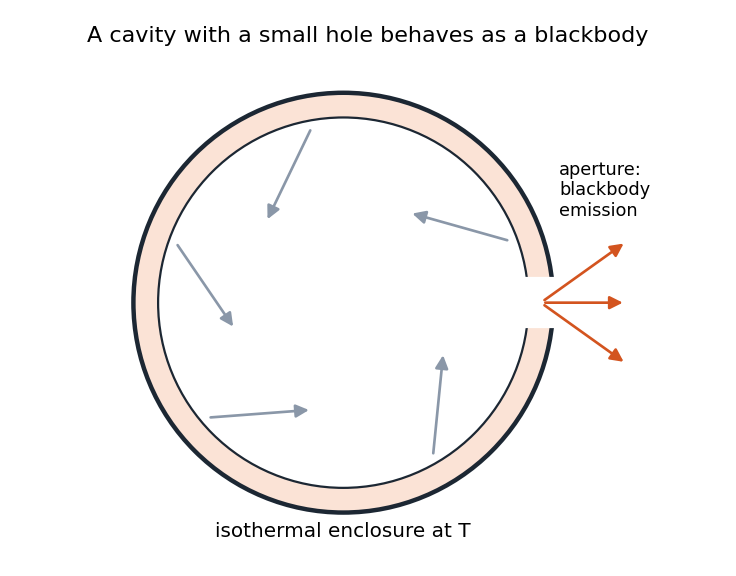
\includegraphics[width=0.5\linewidth]{pics/blackbody_cavity.png}
\end{figure}

%%%%%%%%%%%%%%%%%%%%%%%%%%%%%%%%%%%%%%%%%%%%%%%%%%%%%%%
\subsubsection*{Planck's Distribution}
\addcontentsline{toc}{subsubsection}{Planck's Distribution}
%%%%%%%%%%%%%%%%%%%%%%%%%%%%%%%%%%%%%%%%%%%%%%%%%%%%%%%

The spectral emissive power of a blackbody is described by Planck's distribution:

\begin{definition}
\[
    E_{\lambda,b}(\lambda,T)  = \frac{C_1}{\lambda^5[\exp(C_2/\lambda T)-1]} = \pi I_{\lambda,b}(\lambda,T)
\]

Where:
\begin{align*}
    C_1 &= 2\pi h c_0^2 = 3.742 \times 10^8 \frac{\text{W} \cdot \mu\text{m}^4}{\text{m}^2}
    \\
    C_2 &= \frac{h c_0}{k} = 1.439 \times 10^4 \, \mu\text{m} \cdot \text{K}
    \\
    h &= 6.626 \times 10^{-34} \, \text{J} \cdot \text{s} \quad \text{(Planck's constant)} 
    \\
    k &= 1.381 \times 10^{-23} \, \text{J/K} \quad \text{(Boltzmann's constant)}
    \\
    c_0 &= 2.998 \times 10^8 \, \text{m/s} \quad \text{(speed of light in vacuum)} 
    \\
    T &= \text{absolute temperature [K]}
\end{align*}
\end{definition}

Planck's distribution was a groundbreaking development that:
\begin{itemize}
    \item Initially emerged from curve-fitting experimental data
    \item Led to the concept of energy quantization
    \item Marked the transition from classical to quantum physics
    \item Introduced the quantum theory even before Planck himself fully accepted its implications
\end{itemize}

\subsubsection*{Blackbody Radiation Properties}
\addcontentsline{toc}{subsubsection}{Blackbody Radiation Properties}

The spectral distribution of blackbody radiation has these key characteristics:

\begin{itemize}
    \item The peak wavelength shifts toward shorter wavelengths as temperature increases
    \item The magnitude of the emissive power increases with temperature.
    \item The shape of the spectral distribution remains similar but scales with temperature
    \item Most of the energy is concentrated in certain wavelength ranges
\end{itemize}
%
\begin{figure}[H]
    \centering
    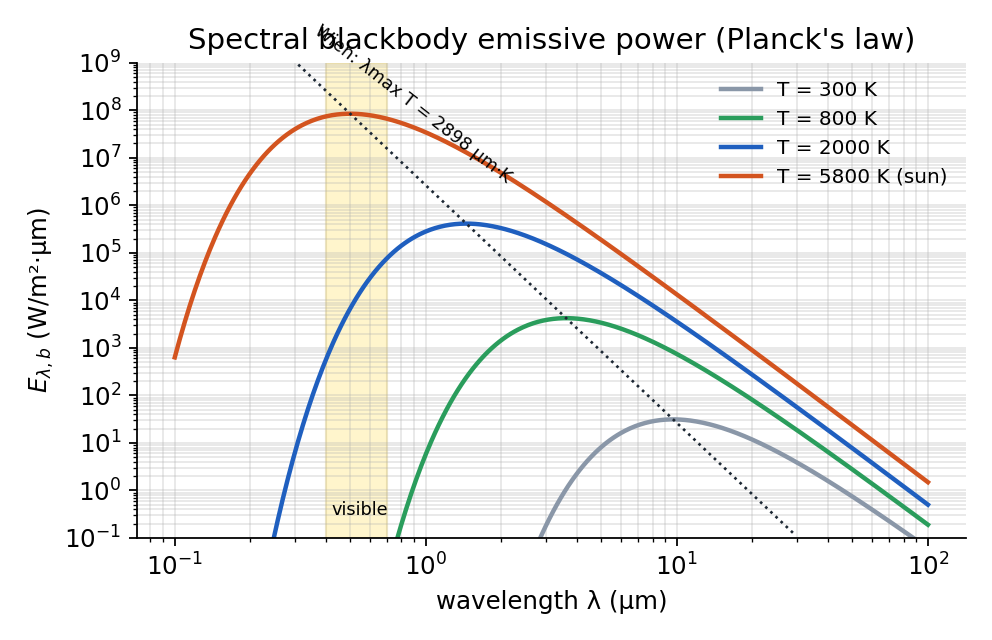
\includegraphics[width=0.4\linewidth]{pics/spectral_blackbodyu_emmisive_power.png}
    \caption{Spectral blackbody emissive power.}
\end{figure}

Planck's law in a few lines (the figure above is this code for several temperatures):
\begin{lstlisting}[language=Python]
import numpy as np
C1, C2 = 3.7418e8, 1.4388e4                  # W um^4/m^2 and um K
def planck(lam_um, T):                       # spectral blackbody emissive power, W/(m^2 um)
    return C1 / (lam_um**5 * (np.exp(C2 / (lam_um * T)) - 1))

lam = np.logspace(-1, 2, 500)
E = planck(lam, 5800)                        # the sun
print(f"peak at {lam[E.argmax()]:.2f} um, Wien predicts {2898/5800:.2f} um")
\end{lstlisting}

%
% For practical calculations:
% \begin{itemize}
%     \item Approximately 1\% of energy is below $\lambda_{max}/2$
%     \item Approximately 75\% of energy is above $\lambda_{max}$
%     \item 99\% of energy falls within the range of $\lambda_{max}/2$ to $8.5\lambda_{max}$
% \end{itemize}

%%%%%%%%%%%%%%%%%%%%%%%%%%%%%%%%%%%%%%%%%%%%%%%%%%%%
\subsubsection*{Stefan-Boltzmann Law}
\addcontentsline{toc}{subsubsection}{Stefan-Boltzmann Law}
%%%%%%%%%%%%%%%%%%%%%%%%%%%%%%%%%%%%%%%%%%%%%%%%%%%%

The total emissive power from a blackbody is obtained by integrating the Planck distribution over all wavelengths:

\begin{definition}
\[
    E_b = \int_0^{\infty} E_{\lambda,b} \, d\lambda = \sigma T^4
\]

Where $\sigma = 5.67 \times 10^{-8}$ W/m$^2$K$^4$ is the Stefan-Boltzmann constant.
\end{definition}
%
This law shows that the total energy emitted by a blackbody increases with the fourth power of its absolute temperature.
%%%%%%%%%%%%%%%%%%%%%%%%%%%%%%%%%%%%%%%%%%%%%%%%%%%%
\subsubsection*{Wien's Displacement Law}
\addcontentsline{toc}{subsubsection}{Wien's Displacement Law}
%%%%%%%%%%%%%%%%%%%%%%%%%%%%%%%%%%%%%%%%%%%%%%%%%%%%

Wien's displacement law gives the wavelength of maximum emission for a blackbody:

\begin{definition}
    \[
        \lambda_{max} \cdot T = C_3 =  2897.8 \, \mu\text{m} \cdot \text{K}
    \]
\end{definition}
This explains why different temperature objects emit radiation in different parts of the spectrum:
\begin{itemize}
    \item Sun ($\approx$ 5800 K): Peak in visible range ($\approx$ 0.5 $\mu$m)
    \item Light bulb ($\approx$ 2900 K): Peak in near infrared ($\approx$ 1.0 $\mu$m)
    \item Room temperature objects ($\approx$ 300 K): Peak in far infrared ($\approx$ 10 $\mu$m)
\end{itemize}

\subsubsection*{Fractional Blackbody Energy Function}
\addcontentsline{toc}{subsubsection}{Fractional Blackbody Energy Function}

For engineering calculations, the fraction of blackbody energy emitted within a wavelength range is useful:

%
\begin{figure}[H]
    \centering
    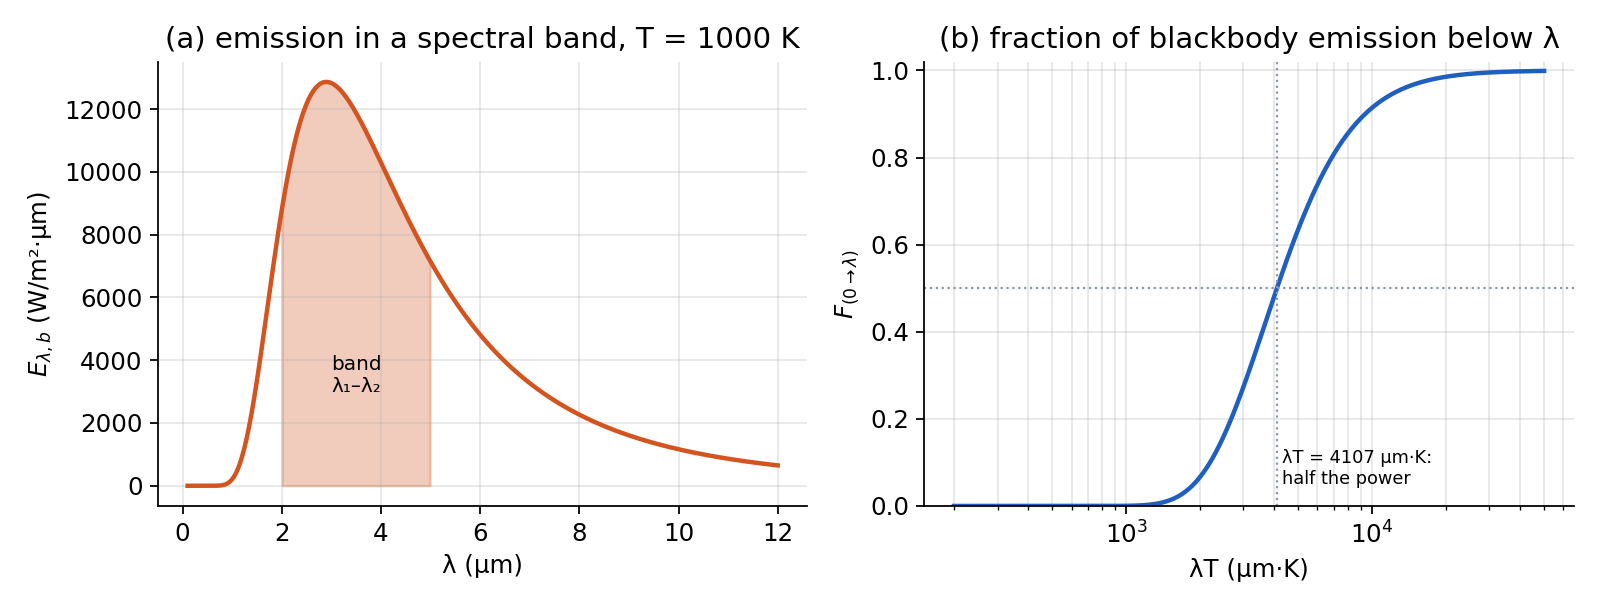
\includegraphics[width=0.7\linewidth]{pics/black_body_prop.png}
    \caption{(a) Radiation emission from a blackbody in the spectral band 0 to $\lambda$, (b) Fraction of the total blackbody emission in the spectral band from 0 to $\lambda$ as a function of $\lambda\, T$}
\end{figure}
%
\begin{definition}

\[
    F_{(0 \rightarrow \lambda)} \equiv \frac{\int_0^\lambda E_{\lambda, b} d \lambda}{\int_0^{\infty} E_{\lambda, b} d \lambda}=\frac{\int_0^\lambda E_{\lambda, b} d \lambda}{\sigma T^4}=\int_0^{\lambda T} \frac{E_{\lambda, b}}{\sigma T^5} d(\lambda T)=f(\lambda T)
\]
\end{definition}
%
This fraction depends only on the product $\lambda T$, and values are tabulated for convenience (Table 12.2 textbook). They may also be used to obtain the fraction of the radiation between any two wavelengths $\lambda_1$ and $\lambda_2$, since

\begin{definition}
\[
    F_{\left(\lambda_1 \rightarrow \lambda_2\right)}=\frac{\int_0^{\lambda_2} E_{\lambda, b} d \lambda-\int_0^{\lambda_1} E_{\lambda, b} d \lambda}{\sigma T^4}=F_{\left(0 \rightarrow \lambda_2\right)}-F_{\left(0 \rightarrow \lambda_1\right)}
\]
\end{definition}

\paragraph{Example:} Find the efficiency of a light bulb with a tungsten filament at 2900 K, visible in range of $350-750$ nm (assume the filament is a blackbody).

\textbf{}

\textit{solution:}
\[
        \eta = \frac{\text{usable E}}{\text{Total E}} = \frac{\text{visible portion}}{\text{Total E}}
\]
For a filament at 2900 K:
\begin{itemize}
    \item Peak wavelength $\approx$ 1.45 $\mu$m (infrared)
    \item Visible range: 350-750 nm = 0.35-0.75 $\mu$m
    \item $\lambda_1 T = 0.35 \times 2900 = 1015$ $\mu\, m\,K$
    \item $\lambda_2 T = 0.75 \times 2900 = 2175$ $\mu\, m\,K$
\end{itemize}

From blackbody fraction tables, the efficiency is approximately:
\[
    \begin{aligned}
        \eta & = \frac{\text{visible portion}}{\text{Total E}} =  F_{(0 \rightarrow \lambda_2)} - F_{(0 \rightarrow \lambda_1)}
        \\[1em]
        & = 0.013754-0.000008
        \\[1em]
        &\approx 0.01375 \text{ or } 1.375\%
    \end{aligned}
\]

This low efficiency is typical for incandescent bulbs, which emit most energy as heat rather than visible light.

%%%%%%%%%%%%%%%%%%%%%%%%%%%%%%%%%%%%%%%%%%%%%%%%%%%%
\subsection*{Emission from Real Surfaces}
\addcontentsline{toc}{subsection}{Emission from Real Surfaces}
%%%%%%%%%%%%%%%%%%%%%%%%%%%%%%%%%%%%%%%%%%%%%%%%%%%%

Real surfaces emit less radiation than blackbodies at the same temperature. Emissivity quantifies this relationship:
%
\[
    \text{Emissivity} = \frac{\text{Radiation emitted by real surface}}{\text{Radiation emitted by blackbody at same temperature}}
\]
%
\begin{figure}[H]
    \centering
    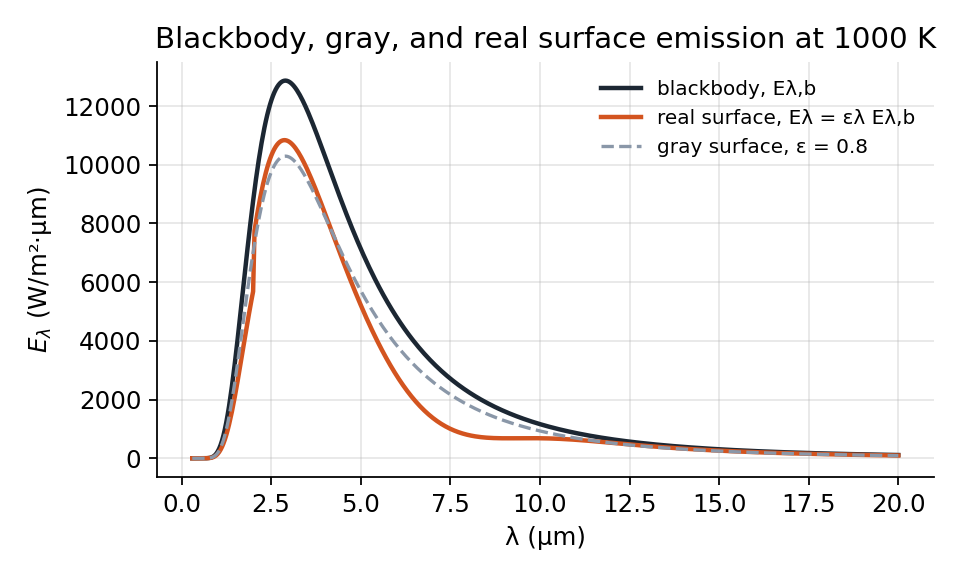
\includegraphics[width=0.32\linewidth]{pics/emission_from_real_surfacew.png}
    \caption{Comparison of spectral distribution of blackbody and real surface emission.}
\end{figure}
%


\subsubsection*{Types of Emissivity}
\addcontentsline{toc}{subsubsection}{Types of Emissivity}

Similar to absorptivity, emissivity can be defined at different levels:
\begin{enumerate}[(i)]
    \item Spectral, directional emissivity:
    \[
    \varepsilon_{\lambda,\theta}(\lambda,\theta,\phi,T_s) = \frac{I_{\lambda,e}(\lambda,\theta,\phi,T_s)}{I_{\lambda,b}(\lambda,T_s)}
    \]
    %
    \item Total directional emissivity:
    \[
    \varepsilon_{\theta}(\theta,\phi,T_s) = \frac{I_e(\theta,\phi,T_s)}{I_b(T_s)}
    \]
    %
    \item Spectral, hemispherical emissivity:
    \[
    \varepsilon_{\lambda}(\lambda,T_s) = \frac{E_{\lambda}(\lambda,T_s)}{E_{\lambda,b}(\lambda,T_s)}
    \]
    %
    \item Total, hemispherical emissivity:
    \textbf{}
    \begin{definition}
    \[
        \varepsilon(T_s)  =\frac{\int_0^{\infty} \varepsilon_\lambda E_{b, \lambda}(T) d \lambda}{\int_0^{\infty} E_{b, \lambda}(T) d \lambda}= \frac{E(T_s)}{E_b(T_s)}
    \]
    this total emissivity is intrinsic surface properties. If we are given emmisivity vs wavelength where the integration may be performed in parts:
    %
    \begin{figure}[H]
        \centering
        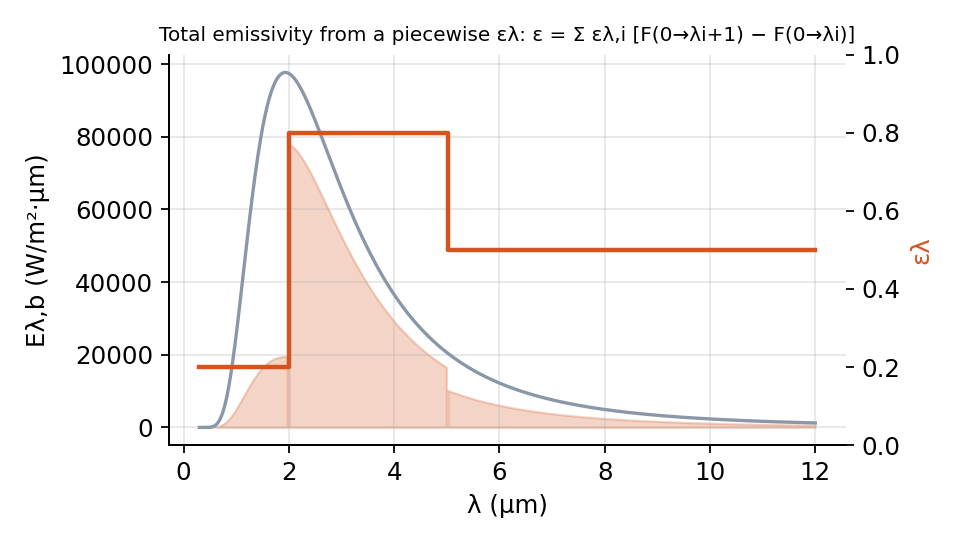
\includegraphics[width=0.5\linewidth]{pics/diagram-20250501.png}
    \end{figure}
    %
    The total  emmisivity can be found as follows:
    \[
        \varepsilon=\frac{\int_0^{\infty} \varepsilon_\lambda E_{\lambda, b} d \lambda}{E_b}=\frac{\varepsilon_1 \int_0^{\lambda_1} E_{\lambda, b} d \lambda}{E_b}+\frac{\varepsilon_2 \int_{\lambda_1}^{\lambda_2} E_{\lambda, b} d \lambda}{E_b} + \cdots
    \]
    which can be simplified to
    \[
        \varepsilon=\varepsilon_1 F_{(0 \rightarrow \lambda_1)}+\varepsilon_2\left[F_{(0 \rightarrow \lambda_2 )}-F_{(0 \rightarrow \lambda_1)}\right] + \cdots
    \]
    Each $F_{0\to \lambda_j}$ can be find using the table at $\lambda_j T_{surface}$.
    \end{definition}
\end{enumerate}
%
\subsubsection*{Emissivity Characteristics}
\addcontentsline{toc}{subsubsection}{Emissivity Characteristics}

General trends in material emissivity:
\begin{itemize}
    \item Metals typically have low emissivity, especially if polished (due to high electron mobility)
    \item Dielectrics (oxides, ceramics) typically have high emissivity
    \item Non-conductors have high emissitivity ($\varepsilon > 0.6$)
    \item Emissivity varies with angle - typically constant near normal, dropping near grazing angles
    \item For engineering calculations, normal emissivity ($\varepsilon_n$) is often a good approximation.
    \[
            \varepsilon = \varepsilon_n,\qquad \qquad \text{when }\theta=0^\circ
    \]
\end{itemize}
%
\begin{figure}[H]
    \centering
    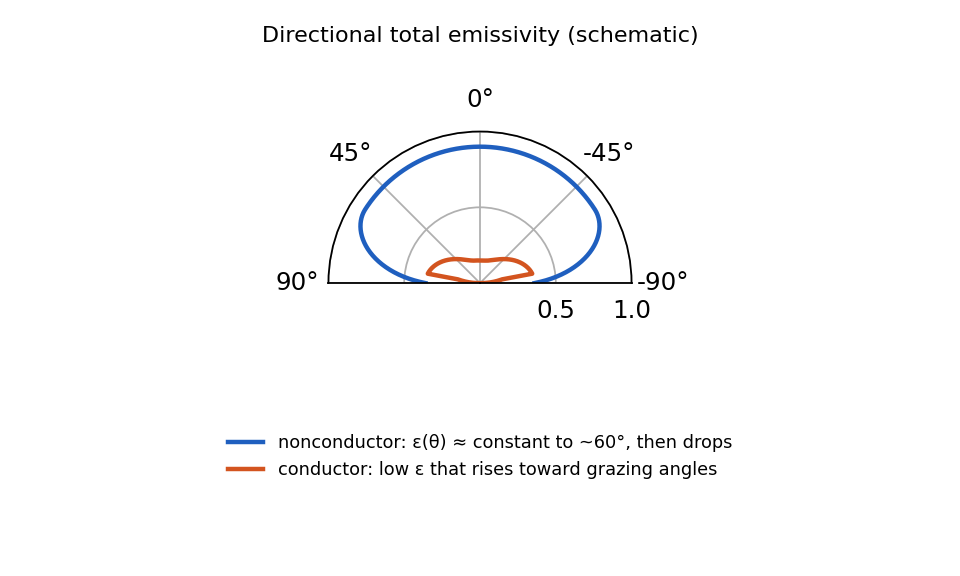
\includegraphics[width=0.45\linewidth]{pics/directional_emmisivity.png}
    \caption{Representative directional distributions of the total, directional emissivity.}
\end{figure}
%%%%%%%%%%%%%%%%%%%%%%%%%%%%%%%%%%%%%%%%%%%%%%%%%%%%%%%%%%%%%%%%%%%%%%%%%%%%%
\subsubsection*{Radiative Properties}
\addcontentsline{toc}{subsubsection}{Radiative Properties}
%%%%%%%%%%%%%%%%%%%%%%%%%%%%%%%%%%%%%%%%%%%%%%%%%%%%%%%%%%%%%%%%%%%%%%%%%%%%%
We define several radiative properties to characterize surface behavior:
%
\paragraph{1. Absorptivity:}
%
\begin{enumerate}[(i)]
    \item Spectral, directional absorptivity:
    \[
    \alpha_{\lambda,\theta}(\lambda,\theta,\phi) = \frac{I_{\lambda,i,\text{abs}}(\lambda,\theta,\phi)}{I_{\lambda,i}(\lambda,\theta,\phi)}
    \]

    \item Spectral, hemispherical absorptivity:
    \[
    \alpha_{\lambda} = \frac{G_{\lambda,\text{abs}}(\lambda)}{G_{\lambda}(\lambda)}
    \]

    \item     Total, hemispherical absorptivity:
    \textbf{}
    \begin{definition}    
    \[
    \alpha = \frac{\displaystyle\int_0^{\infty} \alpha_\lambda(\lambda) G_\lambda(\lambda) d \lambda}{\displaystyle\int_0^{\infty} G_\lambda(\lambda) d \lambda} = \frac{\displaystyle\int_0^{\infty} \alpha_\lambda(\lambda) G_\lambda(\lambda) d \lambda}{G} = \frac{G_{abs}}{G}
    \]
    
    \textbf{}
    
    \textit{Note: } If graph of $G_\lambda$ is given and $\alpha_\lambda$ is constant in different intervals, then we can easily integrate. 
    
    \textbf{}
    
    \textit{Note 2: }If $G_\lambda$ is not given $\alpha_\lambda$ is constant in different intervals, but surface is irradiated by large opaque enclosure, then we know $G_\lambda = E_{b,\lambda}$ so we can use fractional functions $F$ at $(\lambda_i T_{surr})$.
    \end{definition}

\end{enumerate}
%
\paragraph{2. Reflectivity:}
\begin{enumerate}[(i)]
    \item Spectral, directional reflectivity:
    \[
    \rho_{\lambda,\theta}(\lambda,\theta,\phi) = \frac{I_{\lambda,i,\text{ref}}(\lambda,\theta,\phi)}{I_{\lambda,i}(\lambda,\theta,\phi)}
    \]
    %
    \item Spectral, hemispherical reflectivity:
    \[
    \rho_{\lambda} = \frac{G_{\lambda,\text{ref}}(\lambda)}{G_{\lambda}(\lambda)}
    \]
    %
    
    \item  Total, hemispherical reflectivity:
    \textbf{}
    \begin{definition}
    \[
     \rho  = \frac{\displaystyle\int_0^{\infty} \rho_\lambda(\lambda) G_\lambda(\lambda) d \lambda}{\displaystyle\int_0^{\infty} G_\lambda(\lambda) d \lambda} = \frac{\displaystyle\int_0^{\infty} \rho_\lambda(\lambda) G_\lambda(\lambda) d \lambda}{G} =\frac{G_{ref}}{G}
    \]
    \end{definition}
\end{enumerate}


\paragraph{3. Transmissivity:}

\begin{enumerate}[(i)]
    \item Spectral, directional transmissivity:
    \[
    \tau_{\lambda,\theta}(\lambda,\theta,\phi) = \frac{I_{\lambda,i,\text{tr}}(\lambda,\theta,\phi)}{I_{\lambda,i}(\lambda,\theta,\phi)}
    \]
    
    \item Spectral, hemispherical transmissivity:
    \[
    \tau_{\lambda} = \frac{G_{\lambda,\text{tr}}(\lambda)}{G_{\lambda}(\lambda)}
    \]
    \item Total, hemispherical transmissivity:
    \textbf{}
    \begin{definition}    
    \[
    \tau = \frac{\displaystyle\int_0^{\infty} \tau_\lambda(\lambda) G_\lambda(\lambda) d \lambda}{\displaystyle\int_0^{\infty} G_\lambda(\lambda) d \lambda} = \frac{\displaystyle\int_0^{\infty} \tau_\lambda(\lambda) G_\lambda(\lambda) d \lambda}{G} = \frac{G_{trs}}{G}
    \]
    \end{definition}
\end{enumerate}
%%%%%%%%%%%%%%%%%%%%%%%%%%%%%%%%%%%%%%%%%%%%%%%%%%%%
\subsubsection*{Conservation Relationships}
\addcontentsline{toc}{subsubsection}{Conservation Relationships}
%%%%%%%%%%%%%%%%%%%%%%%%%%%%%%%%%%%%%%%%%%%%%%%%%%%%
For all radiative interactions, the conservation of energy requires:

\begin{definition}[Semi-transparent media]
\[
\rho_{\lambda} + \alpha_{\lambda} + \tau_{\lambda} = 1 \quad \text{(spectral)}
\]
\[
\rho + \alpha + \tau = 1 \quad \text{(total)}
\]
\end{definition}

%
\begin{definition}[Opaque media]
\[
\rho_{\lambda} + \alpha_{\lambda} = 1 \quad \text{(spectral)}
\]
\[
\rho + \alpha = 1 \quad \text{(total)}
\]
\end{definition}
% %%%%%%%%%%%%%%%%%%%%%%%%%%%%%%%%%%%%%%%%%%%%%%%%%%%%
% \subsection*{Kirchhoff's Law}
% \addcontentsline{toc}{subsection}{Kirchhoff's Law}
% %%%%%%%%%%%%%%%%%%%%%%%%%%%%%%%%%%%%%%%%%%%%%%%%%%%%

% % Kirchhoff's law establishes a fundamental relationship between emissivity and absorptivity. Consider a surface in an isothermal enclosure at thermal equilibrium:

% % \begin{itemize}
% %     \item For energy balance at equilibrium, absorption must equal emission
% %     \item This leads to the conclusion that $\varepsilon = \alpha$ at thermal equilibrium
% % \end{itemize}

% % This can be mathematically shown through energy balance:
% % \[
% % \alpha \cdot G \cdot A - E \cdot A = 0
% % \]

% % With $G = E_b$ in an isothermal enclosure, we get:
% % \[
% % \alpha E_b = E
% % \]

% % Since $\varepsilon = \frac{E}{E_b}$, we conclude:
% % \[
% % \varepsilon = \alpha
% % \]

% Kirchhoff's law establishes a fundamental relationship between emissivity and absorptivity. Consider a large isothermal enclosure (temperature $T_s$) containing small bodies ($A_1$, $A_2$, $A_3$). This enclosure is called blackbody cavity ($\varepsilon=1$). These bodies are too small to affect the radiation field.

% \textbf{}

% Under these conditions:
% \begin{itemize}
%     \item The irradiation is $G = E_b(T_s) = \sigma T_s^4$
%     \item At thermal equilibrium, all surfaces reach the same temperature: $T_1 = T_2 = T_3 = T_s$
% \end{itemize}
% %
% Considering energy balance on body $A_1$:
% \[
%     \begin{aligned}
%         \dot{E}_{\text {in }}+ \cancelto{0}{\dot{E}_{\text{gen}}}-\dot{E}_{\text {out }} &= \cancelto{0}{\dot{E}_{\text {st }}}
%         \\[0.5em]
%         \alpha_1 \cdot G \cdot A_1 - E_1(T_s) \cdot A_1 &= 0
%         \\[0.5em]
%         \alpha_1 E_b(T_s) &= E_1(T_s)
%     \end{aligned}
% \]
% %
% Since emissivity is defined as $\varepsilon_1 = \frac{E_1}{E_b}$, we conclude $\varepsilon_1 = \alpha_1$. Considering all bodies:
% \[
%     \varepsilon_1 = \alpha_1, \quad \varepsilon_2 = \alpha_2, \quad \varepsilon_3 = \alpha_3
% \]

% Therefore, at isothermal conditions:
% \[
%     \varepsilon = \alpha
% \]
% %%%%%%%%%%%%%%%%%%%%%%%%%%%%%%%%%%%%%%%%%%%%%%%%%%%%
% \subsubsection*{Extensions of Kirchhoff's Law}
% \addcontentsline{toc}{subsubsection}{Extensions of Kirchhoff's Law}
% %%%%%%%%%%%%%%%%%%%%%%%%%%%%%%%%%%%%%%%%%%%%%%%%%%%%
% Kirchhoff's law can be extended to various conditions:

% \begin{enumerate}
%     \item In its most fundamental form, $\varepsilon_{\lambda,\theta} = \alpha_{\lambda,\theta}$ at any surface temperature (inherent surface property)
    
%     \item If irradiation is diffuse OR the surface is diffuse:
%     \[
%     \varepsilon_{\lambda} = \alpha_{\lambda}
%     \]
    
%     \item If irradiation corresponds to that of a blackbody at the surface temperature, OR if the surface is \textbf{gray}\footnote{We will discuss it later. For short, energy of gray materials are independent of $\lambda$.} and conditions for (2) hold:
%     \[
%     \varepsilon = \alpha
%     \]
% \end{enumerate}

% These relationships are extremely useful for simplifying radiation heat transfer analysis.

%%%%%%%%%%%%%%%%%%%%%%%%%%%%%%%%%%%%%%%%%%%%%%%%%%%%
% Irradiation Approximation and Kirchhoff’s Law Notes
%%%%%%%%%%%%%%%%%%%%%%%%%%%%%%%%%%%%%%%%%%%%%%%%%%%%
\subsection*{Large opaque isothermal enclosure}
\addcontentsline{toc}{subsection}{Large opaque isothermal enclosure}
For a large opaque isothermal enclosure, we can apply a useful simplification:

    \begin{itemize}
        \item For any point within the enclosure, radiosity equals irradiation: $J = G$
        \item The black body emission equals both radiosity and irradiation: $E_b = G = J$
        \[
            \begin{aligned}
                &J =\varepsilon E_b+ \rho G
                \\[0.5em]
                &J = \textcolor{red}{(1-\rho)} E_b+ \rho G
                \\[0.5em]
                &J  = (1-\rho) E_b+\rho G
            \end{aligned}
        \]
     we know $J=G$ so
     \[
        \begin{aligned}
            &(1-\rho) E_b+\rho G = G
            \\[0.5em]
            & (1-\rho) E_b  =(1-\rho) G
            \\[0.5em]
            & E_b  =G=J = \sigma T_{surr}^4
        \end{aligned}
     \]
    \end{itemize}
    
    This means that regardless of the actual surface properties, we can treat the enclosure as having an effective emissivity of 1 (black body) for calculation purposes. This concept is sometimes called a "black body cavity" or "black cavity" and is used in practical applications and in deriving Kirchhoff's Law.

    \textbf{
    }

    \textit{Note:} This approximation is also valid  when the surroundings are \textbf{high‑emissivity} (nearly black, $\varepsilon\!\approx\!1$) like Sun is considered as a black body.
%\subsection*{Irradiation Approximation}
% \addcontentsline{toc}{subsection}{Irradiation Approximation}
% A surface receives the \emph{irradiation} $G$ from all directions in the hemisphere above it.  When the surroundings behave like a single blackbody at a uniform temperature~$T_{surr}$, the irradiation can be estimated by
% \[
%   G \approx \sigma T_{surr}^{4}.
% \]
% This approximation is valid whenever
% \begin{itemize}
%   \item the surroundings are \textbf{high‑emissivity} (nearly black, $\varepsilon\!\approx\!1$);
%   \item the surface’s view of those surroundings is \textbf{almost complete} (view‑factor sum $\approx1$); and
%   \item all visible surroundings share the same temperature $T_{surr}$.
% \end{itemize}
% Typical examples include a small test body deep inside a large isothermal cavity or a component facing an extensive, high‑$\varepsilon$ furnace wall held at $T_{surr}$.
%


%%%%%%%%%%%%%%%%%%%%%%%%%%%%%%%%%%%%%%%%%%%%%%%%%%%%
\subsection*{Kirchhoff’s Law}
\addcontentsline{toc}{subsection}{Kirchhoff’s Law}

\paragraph{Fundamental statement}
At each wavelength $\lambda$ and direction $(\theta,\phi)$,
\[
  \varepsilon_{\lambda,\theta,\phi}(T)=\alpha_{\lambda,\theta,\phi}(T).
\]
%
There are several conditions:
\begin{enumerate}[(1)]
    \item \textbf{Diffuse surface or diffuse irradiation}
    If the emission/irradiation is direction‑independent (diffuse) then
    \[
      \varepsilon_{\lambda}(T)=\alpha_{\lambda}(T)
    \]
    \item \textbf{Large opaque isothermal enclosure with $T_s=T_{surr}$}
    In this special rare case, we also have
    \[
            \varepsilon =\alpha
    \]
    
    %
    \item \textbf{Gray surface}
        We can assume $\varepsilon$ and $\alpha$ are wavelength independent:
        \[
            \left\{\begin{aligned}
                \varepsilon_{\lambda} &=\varepsilon_0
                \\[0.5em]
                \alpha_{\lambda} &=\alpha_0        
            \end{aligned}\right.
        \] 
        This is never universal, but a good approximation over small wavelength bands; useful for treating interacting surfaces at similar $T$.
        %
        \begin{figure}[H]
            \centering
            \begin{tikzpicture}
  % First plot - emissivity
  \draw[-latex] (0,0) -- (0,3) node[left] {$\varepsilon_\lambda$};
  \draw[-latex] (0,0) -- (3,0) node[below] {$\lambda$};
  \draw (0,1) -- (3,1);
  
  % Second plot - absorption coefficient
  \draw[-latex] (5,0) -- (5,3) node[left] {$\alpha_\lambda$};
  \draw[-latex] (5,0) -- (8,0) node[below] {$\lambda$};
  \draw (5,2) -- (8,2);
\end{tikzpicture}
        \end{figure}
        %
        \item \textbf{Diffuse + gray}: As a result of Kirchoff’s Law, $  \varepsilon_{\lambda,\theta,\phi}(T)=\alpha_{\lambda,\theta,\phi}(T)$, at equilibirum:
        \begin{itemize}
            \item If the irradiation is diffuse OR the surface is diffuse
            \item The surface is gray
        \end{itemize}
        Then we have
        \[
                \varepsilon = \alpha
        \]
\end{enumerate}
%


%%%%%%%%%%%%%%%%%%%%%%%%%%%%%%%%%%%%%%%%%%%%%%%%%%%%
\subsection*{Net Radiative Heat Flux for a Diffuse, Opaque Surface}
\addcontentsline{toc}{subsection}{Net Radiative Flux}
Consider a \textbf{diffuse, opaque} surface (transmissivity $\tau=0$) at temperature $T_s$.

\paragraph{Radiosity \(J\)}
Because the surface is opaque, anything not emitted is reflected:
\[
  J = E + G_{ref} = \varepsilon E_b+ \rho G = \underbrace{\varepsilon\sigma T_s^{4}}_{\text{emitted}} + \underbrace{(1-\alpha)G}_{\text{reflected}}.
\]

\paragraph{Net heat flux}
With the approximation $G \approx \sigma T_{surr}^{4}$ the outward net flux is
\[
  q''_{\text{rad,net}} = J - G = \sigma\bigl(\varepsilon T_s^{4} - \alpha T_{surr}^{4}\bigr).
\]

\paragraph{Gray surface or \(T_s=T_{surr}\)}
If \(\varepsilon=\alpha\) (gray assumption, or simply equal temperatures), then
\[
  q''_{\text{rad,net}} = \varepsilon\sigma\bigl(T_s^{4}-T_{surr}^{4}\bigr).
\]
The total rate for area $A$ is \(q_{\text{rad,net}} = q''_{\text{rad,net}}\,A\).


%%%%%%%%%%%%%%%%%%%% SUMMARY TABLE %%%%%%%%%%%%%%%%%%%% 
\textbf{}

\textbf{}

\begin{table}[H]
\centering
\caption{Summary of Kirchhoff’s law, gray, diffuse, black-body, and opaque-surface concepts.}
\footnotesize
\setlength{\tabcolsep}{6pt}
\begin{tabularx}{\linewidth}{@{}p{2.5cm} p{4cm} X@{}}
\toprule
\textbf{Concept}     & \textbf{Equations}                                                                                         & \textbf{Remarks}                                                                                     \\
\midrule
Kirchhoff’s law      
  & $\displaystyle \varepsilon_{\lambda,\theta,\phi}(T)
                  =\alpha_{\lambda,\theta,\phi}(T)$
  & Requires surface and radiation field at the same temperature; ensures emissivity equals absorptivity for all wavelengths and directions. \\

\addlinespace
Gray surface         
  & \makecell[l]{$\displaystyle \varepsilon_{\lambda}\approx \varepsilon_0$\\[0.3em]
                 $\displaystyle \alpha_{\lambda} \approx \alpha_0$}
  & Assumes spectral properties constant over the relevant wavelength range, simplifying integrations when variation is negligible. \\

\addlinespace
Diffuse surface      
  & \makecell[l]{$\displaystyle \varepsilon_{\lambda,\theta,\phi}\approx\varepsilon_{\lambda}$\\[0.3em]
                 $\displaystyle \alpha_{\lambda,\theta,\phi}\approx\alpha_{\lambda}$}
  & Emission and absorption independent of direction (independent of $\theta$ and $\phi$). \\

\addlinespace
Black body           
  & \makecell[l]{$\displaystyle \varepsilon_{\lambda} = \alpha_{\lambda}=1$\\[0.3em]
                 $\displaystyle \Rightarrow\;\varepsilon=\alpha=1,\;\rho=\tau=0$}
  & Ideal emitter/absorber at all $\lambda$, $\theta$, $\phi$; hemispherical emissive power $E_b=\sigma T^4$ comes from integrating radiance over a hemisphere. \\

\addlinespace
Opaque surface       
  & \makecell[l]{$\displaystyle \tau_{\lambda}=0\;\Rightarrow\;\alpha_{\lambda}+\rho_{\lambda}=1$\\[0.3em]
                 Total: $\alpha+\rho=1$}
  & No transmission (all incident radiation is absorbed or reflected); common behavior for solids in the infrared (IR). \\
\bottomrule
\end{tabularx}

\end{table}

